% Opcje klasy 'iithesis' opisane sa w komentarzach w pliku klasy. Za ich pomoca
% ustawia sie przede wszystkim jezyk i rodzaj (lic/inz/mgr) pracy, oraz czy na
% drugiej stronie pracy ma byc skladany wzor oswiadczenia o autorskim wykonaniu.
\documentclass[declaration,shortabstract,polish,inz,masc]{iithesis}
\let\lll\relax
\usepackage[utf8]{inputenc}
\usepackage{fancyhdr}
\usepackage[toc]{appendix}
\usepackage{bookmark}
\usepackage{enumerate}
\usepackage{csvsimple}
\usepackage{float}
\usepackage{amsmath}
\usepackage{mathabx}
\usepackage{enumitem}

\usepackage{pdfpages}

\usepackage{color}

\newlist{interface_descs}{enumerate}{10}
\setlist[interface_descs]{label*=\arabic*.}

\definecolor{bluekeywords}{rgb}{0.13,0.13,1}
\definecolor{greencomments}{rgb}{0,0.5,0}
\definecolor{redstrings}{rgb}{0.9,0,0}

\definecolor{lightgray}{rgb}{.9,.9,.9}
\definecolor{darkgray}{rgb}{.4,.4,.4}
\definecolor{purple}{rgb}{0.65, 0.12, 0.82}

\usepackage{listings}
\lstdefinelanguage{json_comment}{
  keywords={true, false},
  keywordstyle=\color{blue}\bfseries,
  identifierstyle=\color{black},
  sensitive=trues,
  comment=[l]{//},
  morecomment=[s]{/*}{*/},
  commentstyle=\color{purple}\ttfamily,
  stringstyle=\color{blue}\ttfamily,
  morestring=[b]',
  morestring=[b]"
}

\lstset{
  language=json_comment,
  showspaces=false,
  showtabs=false,
  breaklines=true,
  showstringspaces=false,
  breakatwhitespace=true,
  keywordstyle=\color{bluekeywords},
  stringstyle=\color{redstrings},
  basicstyle=\fontsize{9}{10}\ttfamily,
  frame=leftline,
  extendedchars=\true,
  literate={ą}{{\k{a}}}1
           {Ą}{{\k{A}}}1
           {ę}{{\k{e}}}1
           {Ę}{{\k{E}}}1
           {ó}{{\'o}}1
           {Ó}{{\'O}}1
           {ś}{{\'s}}1
           {Ś}{{\'S}}1
           {ł}{{\l{}}}1
           {Ł}{{\L{}}}1
           {ż}{{\.z}}1
           {Ż}{{\.Z}}1
           {ź}{{\'z}}1
           {Ź}{{\'Z}}1
           {ć}{{\'c}}1
           {Ć}{{\'C}}1
           {ń}{{\'n}}1
           {Ń}{{\'N}}1
}
\lstset{inputencoding=ansinew}

\pagestyle{fancy}
\fancyhf{}
\fancyfoot[CO,CE]{\thepage}
\fancyhead[RE]{\leftmark}
\fancyhead[LO]{\rightmark}
\renewcommand{\chaptermark}[1]{\markboth{Tymoteusz Kaczorowski, Instytut Informatyki UWr}{}}
\renewcommand{\sectionmark}[1]{\markright{Wykorzystanie sztucznej inteligencji w symulowaniu zachowań biologicznych}}

\polishtitle{Wykorzystanie sztucznej inteligencji\fmlinebreak w symulowaniu zachowań biologicznych}
\englishtitle{Utilizing artificial intelligence to model biological behaviours}

\author{Tymoteusz Kaczorowski}
\advisor{dr Jakub Kowalski}
\date{14 lutego 2018 r.} % Data zlozenia pracy
\transcriptnum{273882} % Numer indeksu
\advisorgen{dr. Jakuba Kowalskiego} % Nazwisko promotora w dopelniaczu

\polishabstract{TODO: streszczenie}



\begin{document}

\chapter{Wstęp}
W ramach tej pracy stworzyłem grę przedstawiającą uproszczony model środowiska naturalnego, której przeznaczeniem jest testowanie metod sztucznej inteligencji. Aplikacja pozwala kontrolować stan symulacji i obserwować, jak AI uczy się grać optymalnie.

Agentem w tej grze jest osiołek, którego zadaniem jest przeżycie odżywiając się ostem. Poczynaniami osiołka kieruje kontroler oparty o algorytm Q-learning \cite{wiki:Qlearning}, który jest odmianą uczenia ze wzmocnieniem (ang. \textit{reinforcement learning}) \cite{Sutton1998Introduction}. Metoda ta polega na uczeniu się optymalnych zachowań przez analizę nagród i kar płynących z podejmowanych decyzji i jest ważną gałęzią uczenia maszynowego \cite{Sutton1988Learning}.  

Wartymi wspomnienia przykładami zastosowania uczenia ze wzmocnieniem są na przykład TD-Gammon \cite{Tesauro1994TDGammon}, który nauczył się grać w grę Backgammon w oparciu o jedynie wyniki gier rozgrywanych z samym sobą, czy AlphaGo, który w 2016 roku był najlepszym programem grającym w Go \cite{Silver2016Mastering}, a jego ostatnia wersja korzystająca z czystego RL (bez wiedzy ludzkich ekspertów wykorzystywanej przez wersję z 2016) wygrywa z poprzednią 100 na 100 gier \cite{silver2017mastering}. Innym znanym zastosowaniem uczenia ze wzmocnieniem jest gra w szachy -- przykładem jest program KnightCap wykorzystujący algorytm TDLeaf($\lambda$) \cite{Baxter2000Learning}.


\section{Motywacja}
Założeniem projektu było stworzenie symulacji inspirowanej światem rzeczywistym, w której egzystują byty zdolne do nauczenia się strategii pozwalającej na optymalne funkcjonowanie. Stworzony model powinien nie tylko pozwolić sztucznej inteligencji na naukę, ale też, po nauczeniu, pozwalać na zaobserwowanie ciekawych zachowań.


\section{Realizacja}
Na potrzeby realizacji celu powstały trzy elementy:

\begin{enumerate}
    \item Środowisko graficzne służące do wizualnego reprezentowania i kontrolowania symulacji
    \item Silnik symulacji, będący grą dla jednego gracza, w której osiołek (gracz) ma za zadanie przeżyć jak najdłużej odżywiając się roślinami
    \item Ucząca się sztuczna inteligencja kontrolująca osiołka
\end{enumerate}

\section{Narzędzia}
Projekt w całości został zrealizowany w języku C\# z wykorzystaniem silnika WPF do części wizualnej.



\chapter{Zasady symulacji}
Symulacja stworzona na potrzeby tej pracy to prosta, turowa gra dla jednego gracza rozgrywająca się na ciągłej, dwuwymiarowej, kwadratowej planszy, na której żyje osiołek. Osiołek musi odżywiać się ostem by przeżyć, lecz poruszanie się po planszy go męczy, powodując dodatkowe zapotrzebowanie na pożywienie.

\section{Byty}
Wszystkie byty posiadają następujące cechy:
\begin{enumerate}    
    \item Pozycja na planszy
    \item Identyfikator
\end{enumerate}

\subsection{Osiołek}
Osiołek jest bytem kontrolowanym przez gracza. W danej turze na planszy znajduje się dokładnie jeden osiołek. Osiołek posiada następujące cechy zdefiniowane w ustawieniach [sekcja \ref{fig:example_settings}]:
\begin{enumerate}    
    \item \textbf{Mass} -- masa, która opisuje stopień wypełnienia żołądka i umożliwiająca osiołkowi funkcjonowanie poprzez spalanie jej
    \item \textbf{MovementSpeed} -- maksymalny dystans, który może pokonać w ciągu tury
    \item \textbf{InteractionDistance} -- zasięg, na którym możliwe jest jedzenie ostu
    \item \textbf{BiteSize} -- maksymalna masa, którą może przyswoić z rośliny w ciągu tury
    \item \textbf{StomachCapacity} -- maksymalny rozmiar żołądka
    \item \textbf{SightRange} -- zasięg, w którym inne byty są dla osiołka widoczne
    \item \textbf{PassiveWork} -- ilość masy zużywanej co turę
    \item \textbf{MovementWork} -- ilość masy zużywanej na potrzeby ruchu 
\end{enumerate}

\subsection{Oset}
Osiołek żywi się ostem. Na planszy może znajdować się co najwyżej określona w ustawieniach symulacji liczba roślin. Każdy oset ma nastepujące cechy:
\begin{enumerate}    
    \item \textbf{Mass} -- określa ilość dostępnego pożywienia w danej roślinie
    \item \textbf{MaxMass} -- maksymalna masa, do której roślina może urosnąć
    \item \textbf{RegrowthRate} -- stały przyrost masy na turę
\end{enumerate}
Maksymalna masa i przyrost masy na turę danej rośliny są losowane z rozkładem jednostajnym na przedziałach zdefiniowanych w ustawieniach [sekcja \ref{fig:example_settings}]. Początkowa masa ostu równa jest jego masie maksymalnej.

\section{Początek gry}
Przed pierwszą turą w losowych miejscach tworzone jest tyle roślin, ile wskazują ustawienia. Następnie w losowym miejscu umieszczany jest osiołek, którego początkowa masa wynosi połowę maksymalnej.

\section{Przebieg gry}
Każda tura przebiega następująco:
\begin{enumerate}    
    \item Wszystkie rośliny, których obecna masa jest większa niż zero zwiększają swoją masę w oparciu o \textbf{RegrowthRate}, nie przekraczając \textbf{MaxMass}.
    \item Wszyskie byty, których masa nie przekracza zera umierają i znikają. Jeśli umiera osiołek symulacja jest resetowana.
    \item Osiołek otrzymuje opis otoczenia i swojego stanu.
    \item Kontroler wybiera akcję dla osiołka w oparciu o ten opis.
    \item Osiołek wykonuje akcję i spala część swojej masy określoną wzorem:

     $\textbf{PassiveWork} + \textbf{MovementWork} \cdot \frac{\textit{distance}}{\textbf{MovementSpeed}}$, gdzie \textit{distance} to dystans przebyty w danej turze.
    \item Jeżeli liczba roślin na planszy nie przekracza maksymalnej, w losowym miejscu na planszy pojawia się nowa roślina, nie częściej niż raz na liczbę tur opisaną w ustawieniach.
\end{enumerate}

\section{Akcje}
W każdej turze siołek może wykonać jedną z poniższych akcji:
\begin{enumerate}    
    \item Pominięcie tury.
    \item Próba zjedzenia wybranej rośliny, która przekazuje część swojej masy osiołkowi jeśli ten znajduje się w odpowiednim zasięgu. Ilość zaabsorbowanej masy wynosi.
    
    $min(\textbf{BiteSize}, \textbf{plant.Mass}, \textbf{StomachCapacity - donkey.Mass})$
    \item Poruszenie się w stronę zadanego punktu o wybrany dystans z zakresu $[0,\textbf{MovementSpeed}]$.
\end{enumerate}






\chapter{Aplikacja}
Aplikacja udostępnia prostą wizualizację oraz metody kontrolowania i podglądu stanu symulacji. Ten rozdział opisuje interfejs, obsługę i działanie aplikacji.

\section{Działanie aplikacji}
Po uruchomieniu użytkownik proszony jest o wybranie pliku \texttt{.json} z ustawieniami. Następnie tworzona jest instancja kontrolera osiołka i uruchamiane są zadania cykliczne: odświeżanie grafiki i obliczanie kolejnych tur symulacji. Program przyjmuje jeden opcjonalny argument wywołania: liczbę całkowitą określającą liczbę odświeżeń grafiki na sekundę. Wartość domyślna tego argumentu wynosi 20.

W momencie śmierci osiołka symulacja jest resetowana, ale licznik tur i kontroler zachowują swoje stany.

\clearpage

\section{Opis interfejsu}
\begin{figure}[H]
    \centering
    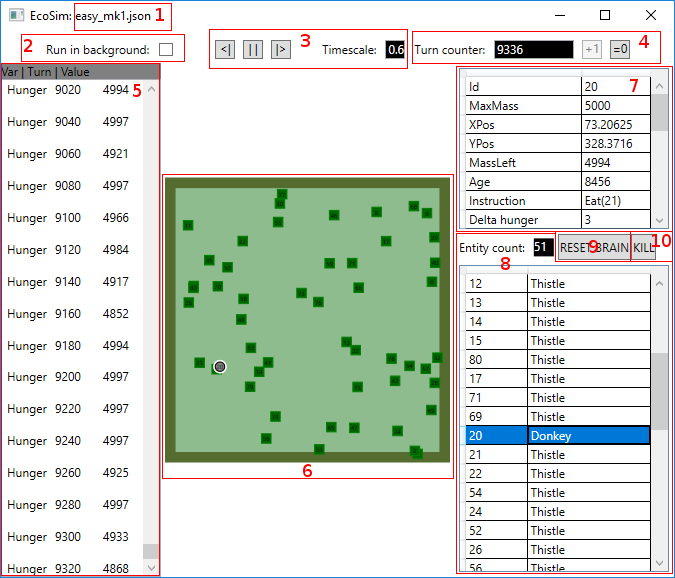
\includegraphics[scale=0.55]{Chapters/interface_annotated}
    \end{figure}
\begin{interface_descs}
    \item Nazwa wybranego pliku z ustawieniami.
    \item Checkbox pozwalający wyłączyć odświeżanie grafiki i obliczać kolejne tury symulacji tak szybko, jak jest to możliwe.
    \item Przyciski kontrolujące częstotliwość obliczania kolejnych tur symulacji.
    \item Licznik tur. Przycisk \textit{+1} pozwala obliczyć kolejną turę symulacji gdy \textbf{Timescale} jest równe 0. Przycisk \textit{=0} resetuje licznik tur.
    \item Log, w którym pojawiają się wiadomości tworzone przez symulację. W przykładzie jest to bieżąca tura i stan żołądka osiołka wypisywane co 20 tur.
    \item Plansza reprezentująca stan symulacji.
    \item Szczegóły obecnie wybranego bytu. Byt można wybrać klikając go na planszy lub na liście bytów.
    \item Lista bytów znajdujących się na planszy.
    \item Przycisk pozwalający wywołać metodę \textit{Reset()} na kontrolerze osiołka, która ponownie inicjalizuje jego stan wartościami początkowymi.
    \item Przycisk pozwalający natychmiastowo zabić obecną instancję osiołka.
\end{interface_descs}

\section{Ustawienia}
Symulacja oraz kontroler są parametryzowane plikiem \texttt{.json}. Poniżej przedstawiam przykładowy plik z ustawieniami oraz ich opisami:
\begin{figure}[h]
\label{fig:example_settings}
\begin{lstlisting}[language=json_comment]
{
"Brain": "Mark1", //"Mark1" lub "Mark0", wybiera rodzaj kontrolera

"LogDeaths" : false, //wartość true sprawia, że po każdej śmierci osiołka zalogowana zostanie tura jego urodzin i wiek w momencie zgonu

"LogHungerEvery": 20, //loguje stan żołądka osiołka co każde LogHungerEvery tur. Wartość 0 wyłącza tę opcję.

"InitialPlantCount": 20, //liczba roślin pojawiająca się na początku symulacji

"MaxPlantCount": 50, //maksymalna liczba roślin na planszy

"NewPlantFrequency": 5, //liczba tur między pojawieniami się nowych roślin

"MinPlantMass": 100, //dolna granica przedziału, z którego losowana jest maksymalna masa rośliny
"MaxPlantMass": 500, //górna granica w/w przedziału

"MinGrowthRate": 30, //dolna granica przedziału, z którego losowany jest parametr RegrowthRate rośliny
"MaxGrowthRate": 50, //górna granica w/w przedziału

// opisane w rozdz. 2 pracy:
"MovementSpeed": 20,         
"InteractionDistance": 22,         
"BiteSize": 100,         
"StomachCapacity": 5000,        
"SightRange": 88, 
"PassiveWork": 3,
"MovementWork": 5,

// opisane w rozdz. 4 pracy:
"BrainBaseActionScore": 0.0022,
"BrainDiscount": 0.6,        
"BrainLearningRate": 0.148,        
"BrainLearningRateDamping": 0.99999,         
"BrainBaseActionScoreDamping" : 0.99952,         
"BrainProbabilityExponent": 1.6 
}
\end{lstlisting}
\end{figure}

\chapter{Sztuczna inteligencja}
Poczynaniami osiołka kieruje kontroler implementujący algorytm Q-learning [TODO: jakieś citation]. W tym rozdziale opiszę szczegóły implementacji kontrolera.

Wybrany algorytm w prosty sposob pozwala na nauczenie się, jakie decyzje podejmować w danym kontekście utrzymując balans między wybieraniem natychmiastowej nagrody, a dążeniem do stanów o większym potencjale zdobycia nagrody, nawet jeśli oznacza to mniejszy zysk krótkofalowy. 

\section{Rodzaje kontrolerów}
Zaimplementowane zostały dwa rodzaje kontrolerów, \textit{Mark1} i \textit{Mark0}. Różnią się jedynie liczbą stanów, które rozróżniają - \textit{Mark0} jest "krótkowzroczny" i nie analizuje pożywienia poza zasięgiem interakcji. \textit{Mark1} uwzględnia w swojej przestrzeni stanów wszystkie rośliny w zasięgu wzroku, największą uwagę zwracając na te, które znajdują się bliżej agenta.

\section{Kwantyzacja stanu}
Kontroler w każdej turze symulacji otrzymuje opis stanu osiołka:
\begin{enumerate}
    \item \textbf{Hunger} - liczba z zakresu 0-1 równa $1-\frac{\textbf{donkey.Mass}}{\textbf{donkey.MaxMass}}$
    \item Pozycję osiołka
    \item Pozycje i masy wszystkich roślin w zasięgu wzroku osiołka
\end{enumerate}
Na potrzeby działania algorytmu stan ten sprowadzany jest do liczby 19-bitowej (11-bitowej dla kontrolera \textit{Mark0}). Składa się na nią kolejno:
\begin{enumerate}
    \item \textbf{Penalty} - liczba 3-bitowa równa $\lfloor\textbf{Hunger}\cdot7\rfloor$
    \item \textbf{FoodRichDirections} - liczba 8-bitowa wyznaczająca kierunki bogate w pożywienie (tylko w kontrolerze \textit{Mark1})
    \item \textbf{CloseFoodDirections} - liczba 8-bitowa wyznaczająca kierunki, w których pożywienie znajduje się w zasięgu interakcji
\end{enumerate}

Kontroler rozróżnia osiem kierunków. Kolejne bity liczb \textbf{FoodRichDirections} i \textbf{CloseRichDirections} wyznaczają kolejne kierunki.

\begin{figure}[H]
    \centering
    4.2. - Rysunek pomocniczy\\
    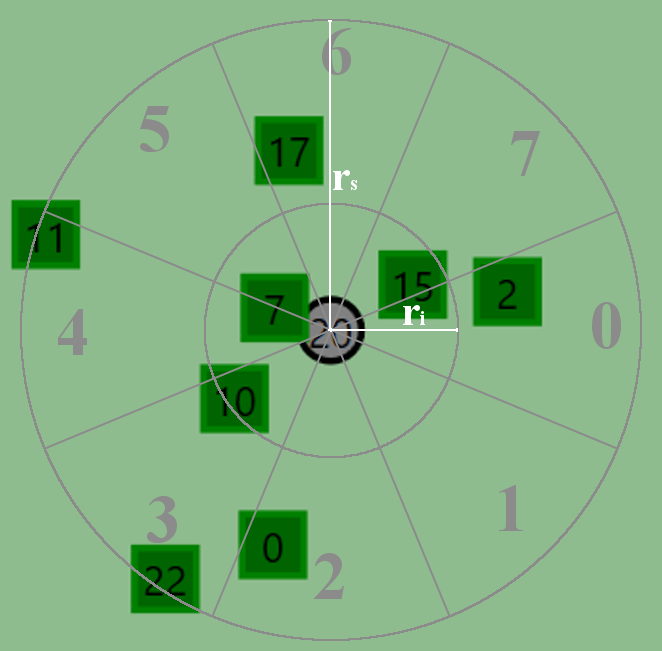
\includegraphics[scale=0.4]{Chapters/vision}
\end{figure}

Niech:
\begin{itemize}
    \item $r_{i}$ oznacza zasięg interakcji
    \item
     $L(a,b)= 
    \begin{cases}
        1,& \text{gdy } a\leq b\\
        0,              & \text{w p. p.}
    \end{cases}
    $
    \item $P_{k,0}...P_{k,n_{k}}$ reprezentuje wszystkie rośliny w zasięgu wzroku ($r_{s}$) w kierunku $k$, $k=0...7$. 
    \item $M(P)$ oznacza masę danej rośliny $P$
    \item $D(P)$ oznacza odległość rośliny $P$ od osiołka
    \item $C_{k} = \sum_{i=0}^{n_{k}} M(P_{k,i}) \cdot L(D(P_{k,i}),r_{i})  $
    \item $C = \sum_{d=0}^{7} C_{d}$
    \item $R'_{k} = \sum_{i=0}^{n_{k}} \frac{M(P_{k,i})}{D(P_{k,i}) - r_{i} + 1} \cdot (1-L(D(P_{k,i}),r_{i})) $
    \item $R_{k} = \frac{R'_{(k-1) \mod 8} + R'_{(k+1) \mod 8}}{2} + R'_{k}$
    \item $R = \sum_{d=0}^{7} R_{d}$
\end{itemize}
\clearpage
Wtedy:
\\$\textbf{CloseFoodDirections} = \sum_{d=0}^{7} 2^{d} \cdot L(\frac{C}{9},C_{d})$
\\$\textbf{FoodRichDirections} = \sum_{d=0}^{7} 2^{d} \cdot L(\frac{R}{9},R_{d})$

Tak więc bit \textbf{CloseFoodDirections} jest równy $1$, jeśli w wyznaczanym przez niego kierunku znajduje się więcej jedzenia w zasięgu interakcji niż przeciętnie. 

Bit \textbf{FoodRichDirections} jest równy $1$, jeśli w wyznaczanym przez niego kierunku, znajduje się poza zasięgiem interakcji (po przeskalowaniu względem odległości i uwzględnieniu kierunków sąsiednich) więcej jedzenia niż przeciętnie.

\section{Akcje}
Instrukcje, które kontroler może wydać osiołkowi są uproszczone, podobnie jak stany. Akcja w rozumieniu kontrolera składa się z dwóch elementów:
\begin{itemize}
    \item Rodzaj - pominięcie tury, ruch, jedzenie
    \item Kierunek - liczba od 0 do 7
\end{itemize}
Akcja taka jest jest po wybraniu tłumaczona na instrukcję w rozumieniu silnika symulacji. Próba zjedzenia obiera na cel najbliższą roślinę w danym kierunku, zaś ruch obiera kierunek odpowiadający zadanemu, dla uproszczenia odchylany w stronę najbliższej rośliny w tym kierunku.

\section{Parametry kontrolera}
Parametry kontrolera definiowane są w pliku .json z ustawieniami. Są to:
\begin{enumerate}
    \item\textbf{ProbabilityExponent} - zwiększa różnicę w prawdopodobieństwie między najlepszymi a najgorszymi akcjami
    \item\textbf{StartLearningRate} - początkowa wartość parametru $\alpha$, który wpływa na skalę zmian wprowadzanych do stanu kontrolera po każdej decyzji
    \item\textbf{LearningRateDamping} - zmniejsza wartość parametru $\alpha$ kontrolera z czasem poprzez mnożenie go przez tę liczbę w każdej turze
    \item\textbf{StartBaseActionScore} - początkowy \textbf{BaseActionScore}, który zapewnia niezerowe prawdopodobieństwo wszystkim możliwym akcjom
    \item\textbf{BaseActionScoreDamping} - zmniejsza faktyczny \textbf{BaseActionScore} kontrolera z czasem poprzez mnożenie go przez tę liczbę w każdej turze
    \item\textbf{Discount} - wartość parametru $\gamma$, który wpływa na balans między rozważaniem natychmiastowej nagrody płynącej z akcji i jej konsekwencji
\end{enumerate}

\section{Nauka}
Kontroler wykorzystuje prosty Q-Learning oparty o tabelkę definiującą funkcję $Q$, która każdej parze (stan,akcja) przyporządkowuje pewną wartość, która jest modyfikowana w czasie nauki. Na początku funkcja ta ma wartość 0 dla wszystkich argumentów.

Przyjmijmy, że w turze $t$ osiołek znajdował się w stanie $S_{t}$, jego \textbf{Hunger} wynosił $H_{t}$ i podjął akcję $A_{t}$. Doprowadziło go to do stanu $S_{t+1}$, w którym \textbf{Hunger} wynosi $H_{t+1}$. Niech $\Delta H = H_{t} - H_{t+1}$, $\alpha_{t} = \textbf{StartLearningRate} \cdot \textbf{LearningRateDamping}^{t}$ Wtedy:
\[Q_{t+1}(s_{t},a_{t})= Q_{t}(s_{t},a_{t}) \cdot (1-\alpha_{t}) + \alpha_{t} \cdot (\Delta H + \gamma \cdot max_{a}Q_{t}(s_{t+1},a))
\]

Dla wszystkich $(s,a)$ różnych od $(s_{t},a_{t})$ $Q_{t+1}(s,a) = Q_{t}(s,a)$

\section{Podejmowanie decyzji}
Po zaktualizowaniu funkcji $Q$ wybierana jest akcja do podjęcia w danej turze. Każda akcja ma pewne pradopodobieństwo zostania wybraną, zależne od wartości funkcji $Q$. Niech $\beta_{t} = \textbf{StartBaseActionScore} \cdot \textbf{BaseActionScoreDamping}^{t}$. Wtedy prawdopodobieństwo akcji $a$ w stanie $s_{t}$ wynosi:

$P_{t}(s_{t},a) = \frac{P'_{t}(s_{t},a)}{\sum_{a'}P'_{t}(s_{t},a')}$, gdzie

$P'_{t}(s_{t},a) = (Q_{t}(s_{t},a) - min_{a'}Q_{t}(s_{t},a') + \beta_{t})^{\textbf{ProbabilityExponent}}$

Parametr $\beta$ zapewnia niezerowe prawdopodobieństwo każdej możliwej akcji, dzięki czemu akcje uznane wcześnie za dobre nie dominują tych jeszcze niewypróbowanych. \textbf{ProbabilityExponent} zwiększa szanse wybrania dobrych akcji zmniejszając szanse wybrania złych.
\chapter{Eksperymenty}
W ramach testów kontrolera przygotowałem kilka zestawów ustawień. W tym rozdziale opiszę, jak zaprojektowana przeze mnie sztuczna inteligencja radzi sobie w różnych środowiskach.

Parametry algorytmu uczącego były dobierane do wymyślonych ustawień świata w sposób eksperymentalny. Ostateczne pliki ustawień uwzględnione w tej pracy zawierają najlepsze z wypróbowanych parametrów.

\section{Ustawienia \textit{simple\_mk1} i \textit{simple\_mk0}}
Te ustawienia tworzą dość prosty świat - osiołek może zadomowić się w pobliżu jednego ostu i odżywiać się nim w nieskończoność, bo w żadnej turze nie zużywa więcej energii, niż najmniejszy możliwy przyrost masy rośliny. I do takiej właśnie strategii dochodzi za każdym razem kontroler \textit{Mark1}.
\begin{figure}[H]
    \centering
    Stan żołądka osiołka względem liczby tur poświęconych na uczenie AI
    \\(częstotliwość próbkowania: raz na 500 tur oraz przy każdym zgonie)
    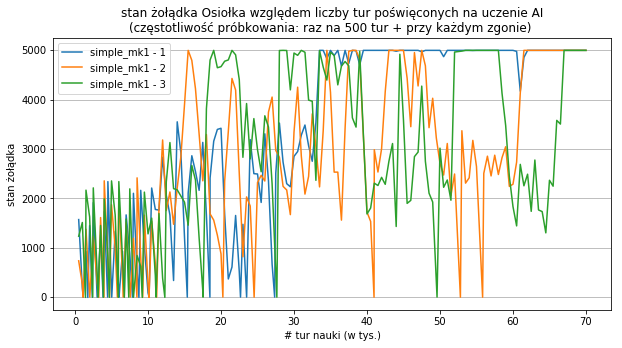
\includegraphics[scale=0.6]{Chapters/simple_mk1_hunger}
\end{figure}

Na wykresie narysowane są trzy łamane odpowiadające trzem różnym uruchomieniom programu z tymi samymi ustawieniami. Każda z nich reprezentuje w istocie wiele instancji osiołka - w momencie osiągnięcia zera symulacja resetuje się, ale kontroler zachowuje wyniesione doświadczenia. 

Z rysunku można wywnioskować, że różne uruchomienia dochodzą do strategii optymalnej w różnym czasie. Mimo to można dostrzec, że z upływem czasu zagęszczenie zgonów się zmniejsza, a wykres zaczyna oscylować w okolicach wyższych wartości. Podobne wnioski można odnieść przy wszystkich innych ustawieniach, więc dla czytelności w następnych wykresach przedstawiał będę tylko dwa uruchomienia.

\begin{figure}[H]
    \centering    
    Stan żołądka osiołka względem liczby tur poświęconych na uczenie AI
    \\(częstotliwość próbkowania: raz na 500 tur oraz przy każdym zgonie)
    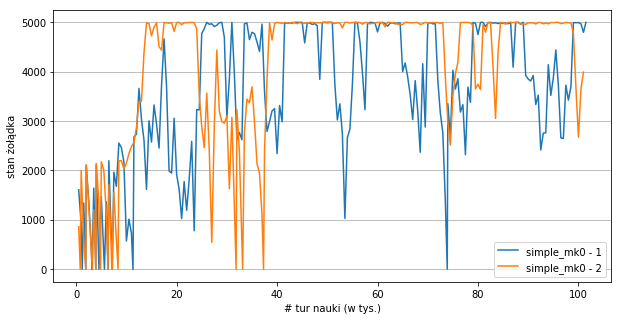
\includegraphics[scale=0.6]{Chapters/simple_mk0_hunger}
\end{figure}

Ten wykres przedstawia dwa uruchomienia z tymi samymi ustawieniami świata dla kontrolera \textit{Mark0}. Ze względu na fakt, że kontroler ten nie analizuje ostów znajdujących się poza zasięgiem interakcji nie dochodzi on do dokładnie tego samego stanu, co \textit{Mark1}. Świat budowany przez te ustawienia nie ma dużego zagęszczenia roślin. Oznacza to, że częstokroć gdy błądzący osiołek w końcu natrafia na jedną zjada ją w całości.

Mimo ograniczeń kontrolera, w każdej próbie uruchomienia programu na tych ustawieniach osiąga on stan, w którym osiołek już więcej nie umiera.

\section{Ustawienia \textit{smallStomach\_mk1} i \textit{smallStomach\_mk0}}
W przypadku tych  ustawień osiołek ma mało czasu na znalezienie pożywienia ze względu na mały rozmiar żołądka i relatywnie duże zużycie energii na turę. Utrudnia to kontrolerowi uczenie się, jednak i tu osiągana jest w pewnym momencie strategia pozwalająca na przeżycie w nieskończoność.

Sprawę ułatwia fakt, że osiołek nigdy nie zjada żadnej rośliny w całości - każda odrasta szybciej, niż ten jest w stanie absorbować jej masę, więc strategia z ustawień \textit{simple} wciąż jest adekwatna.

\begin{figure}[H]
    \centering
    
    Stan żołądka osiołka względem liczby tur poświęconych na uczenie AI
    \\(częstotliwość próbkowania: raz na 700 tur oraz przy każdym zgonie)
    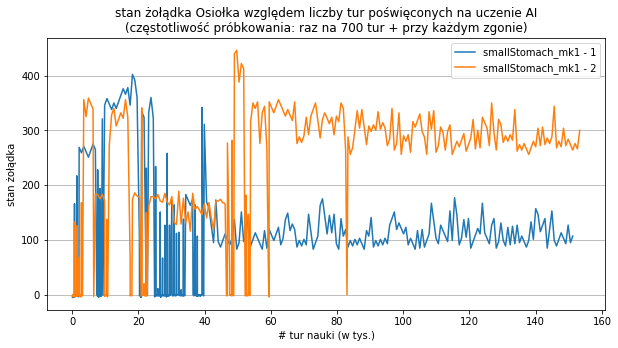
\includegraphics[scale=0.6]{Chapters/smallStomach_mk1_hunger}
\end{figure}

Choć na wykresie można dostrzec trochę mniejsze zagęszczenie zgonów wraz z postępem nauki, kontroler \textit{Mark1} daje wiele podobnie mało satysfakcjonujących żywotów i ostatni, w którym stosuje już efektywną strategię.

Ciekawym jest, że w przeciwieństwie do ustawień \textit{simple} stan żołądka po osiągnięciu stanu ostatecznego może oscylować wokół różnych wartości zależnie od uruchomienia.

\begin{figure}[H]
    \centering
    Stan żołądka osiołka względem liczby tur poświęconych na uczenie AI
    \\(częstotliwość próbkowania: raz na 700 tur oraz przy każdym zgonie)
    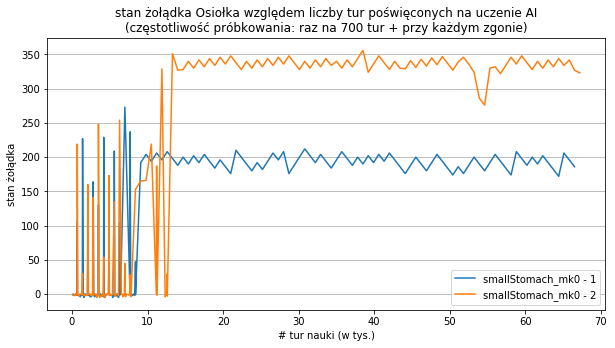
\includegraphics[scale=0.6]{Chapters/smallStomach_mk0_hunger}
\end{figure}

Podobnie jak w przypadku\textit{Mark1}, testy kontrolera \textit{Mark0} nie wykazały dużej tendencji wzrostowej w jakości strategii względem czasu, aż do osiągnięcia strategii pozwalającej na nieśmiertelność. Także i on zależnie od uruchomienia osiąga stany, w których stan żołądka oscyluje wokół różnych wartości.

\textit{Mark0} osiąga jednak strategię efektywną znacznie szybciej - mniejsza liczba rozróżnianych stanów wydaje się być w przypadku tych ustawień zaletą. Analizowanie odległych roślin nie przynosi tu korzyści, za to zwiększa czas potrzebny na naukę.

\section{Ustawienia \textit{oneBite\_mk1}}
To najtrudniejsze z przygotowanych przeze mnie ustawień. Wszystkie rośliny mają jednakową masę, wystarczająco małą by osiołek mógł zjeść je w jednej turze i nie regenerują się. Oznacza to, że zjedzenie rośliny często prowadzi do mało korzystnego stanu, w którym trzeba się przemieścić, by znaleźć kolejną. Trudno zatem znaleźć odpowiednie parametry -- mały \textbf{Discount} prowadzi do kontrolera, który preferuje się nie przemieszczać, zaś duży zmniejsza atrakcyjność jedzenia.

Spośród wszystkich sprawdzonych ustawień \textit{oneBite} daje, po nauczeniu, najciekawszy do obserwowania kontroler, ponieważ zasady świata zmuszają go do nauczenia się, jak radzić sobie w zmiennym środowisku i systematycznie odnajdywać nowe źródła pożywienia, gdy dotychczas wykorzystywane się wyczerpią.
\begin{figure}[H]
    \centering
    Stan żołądka osiołka względem liczby tur poświęconych na uczenie AI
    \\(częstotliwość próbkowania: raz na 1000 tur oraz przy każdym zgonie)
    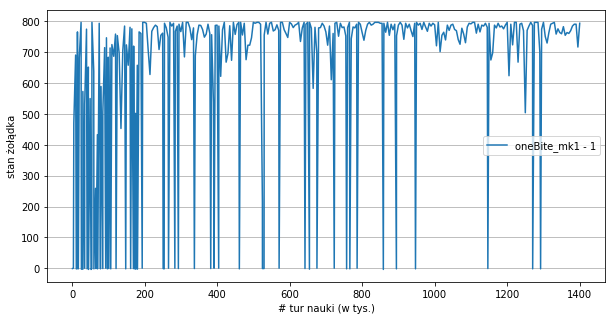
\includegraphics[scale=0.6]{Chapters/oneBite_mk1}
\end{figure}
Tym razem wszystkie uruchomienia dają bardzo podobne wykresy, więc dla czytelności przedstawione zostało tylko jedno. Można dostrzec mniejsze zagęszczenie zgonów wraz z czasem nauki, co sugeruje dążenie do efektywnej strategii. Mimo to w żadnym z wykonanych przeze mnie testów najdłuższy zarejestrowany żywot nie przekraczał 400 tysięcy tur.

Kontroler \textit{Mark0} nie daje dla ustawień \textit{oneBite} satysfakcjonujących wyników - żaden zarejestrowany przeze mnie żywot nie przekroczył 100 tysięcy tur, a zagęszczenie zgonów w czasie nie maleje z czasem.

\chapter{Podsumowanie}
Powstała w skutek tej pracy aplikacja pozwala na tworzenie i obserwowanie wielu symulacji, w których kontroler w różny sposób dąży do innych strategii. Przeprowadzone testy pokazują, że zaimplementowany algorytm istotnie uczy się efektywnych zachowań na przygotowanych przykładach ustawień.

Aplikację można w łatwy sposób rozszerzyć o bardziej rozbudowane zasady symulacji i kontrolery. Dużą część pracy potrzebnej do stworzenia ciekawej symulacji stanowią jednak szukanie odpowiednich ustawień oraz testy, czynność którą można i warto by zautomatyzować.


  \bibliographystyle{plain}
  \bibliography{iithesis} 



\end{document}